\documentclass{standalone}
\usepackage{tikz}
\newcommand{\circulo}[1]{
	\filldraw [fill=blue!40, draw=black] (#1) circle (1.5mm);
	} 
	\newcommand{\cuadro}[1]{
	\filldraw [fill=red!40,draw=black,rotate around = {45:(#1)}] (#1) rectangle ++(0.3,0.3);
	} 
\begin{document}

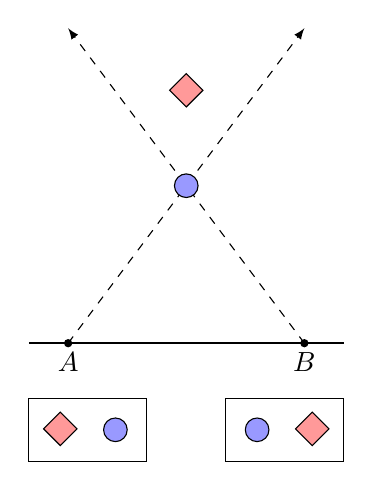
\begin{tikzpicture}[>=latex]
	\draw [thick] (-2,0) -- (2,0);
	\draw [dashed ,->] (-1.5,0) -- (1.5,4);
	\draw [dashed ,->] (1.5,0) -- (-1.5,4);
	\fill (-1.5,0) circle (1.5pt) node [below] {\(A\)};
	\fill (1.5,0) circle (1.5pt) node [below] {\(B\)};
	\circulo{0,2}
	\cuadro{0,3}
	\begin{scope}[yshift=-1.5cm]
		\draw (-2,0) rectangle (-0.5,0.8);
		\circulo{-0.9,0.4}
		\cuadro{-1.6,0.2}
		\draw (2,0) rectangle (0.5,0.8);
		\circulo{0.9,0.4}
		\cuadro{1.6,0.2}
	\end{scope}
\end{tikzpicture}

\end{document}
